\subsection{Statemachine}
\subsubsection{Businesslogik}
Die App besitzt zwei Threads. Der Erste ist nur für die Kommunikation und Interpretation der nsh Kommandos verantwortlich. Dieser Thread läuft nur ein paar Zyklen lang und steuert den zweiten Task. Die Steuerkommandos sind start, stop, status, help.\\

\noindent Der zweite Thread übernimmt die gesammte Businesslogik, welche in Abbildung \ref{fig:Statemachine Businesslogik} aufgezeigt wird. Es werden jeweils Daten zwischen Interfaces ausgetauscht.\\

\begin{figure}[ht]
  \begin{center}
  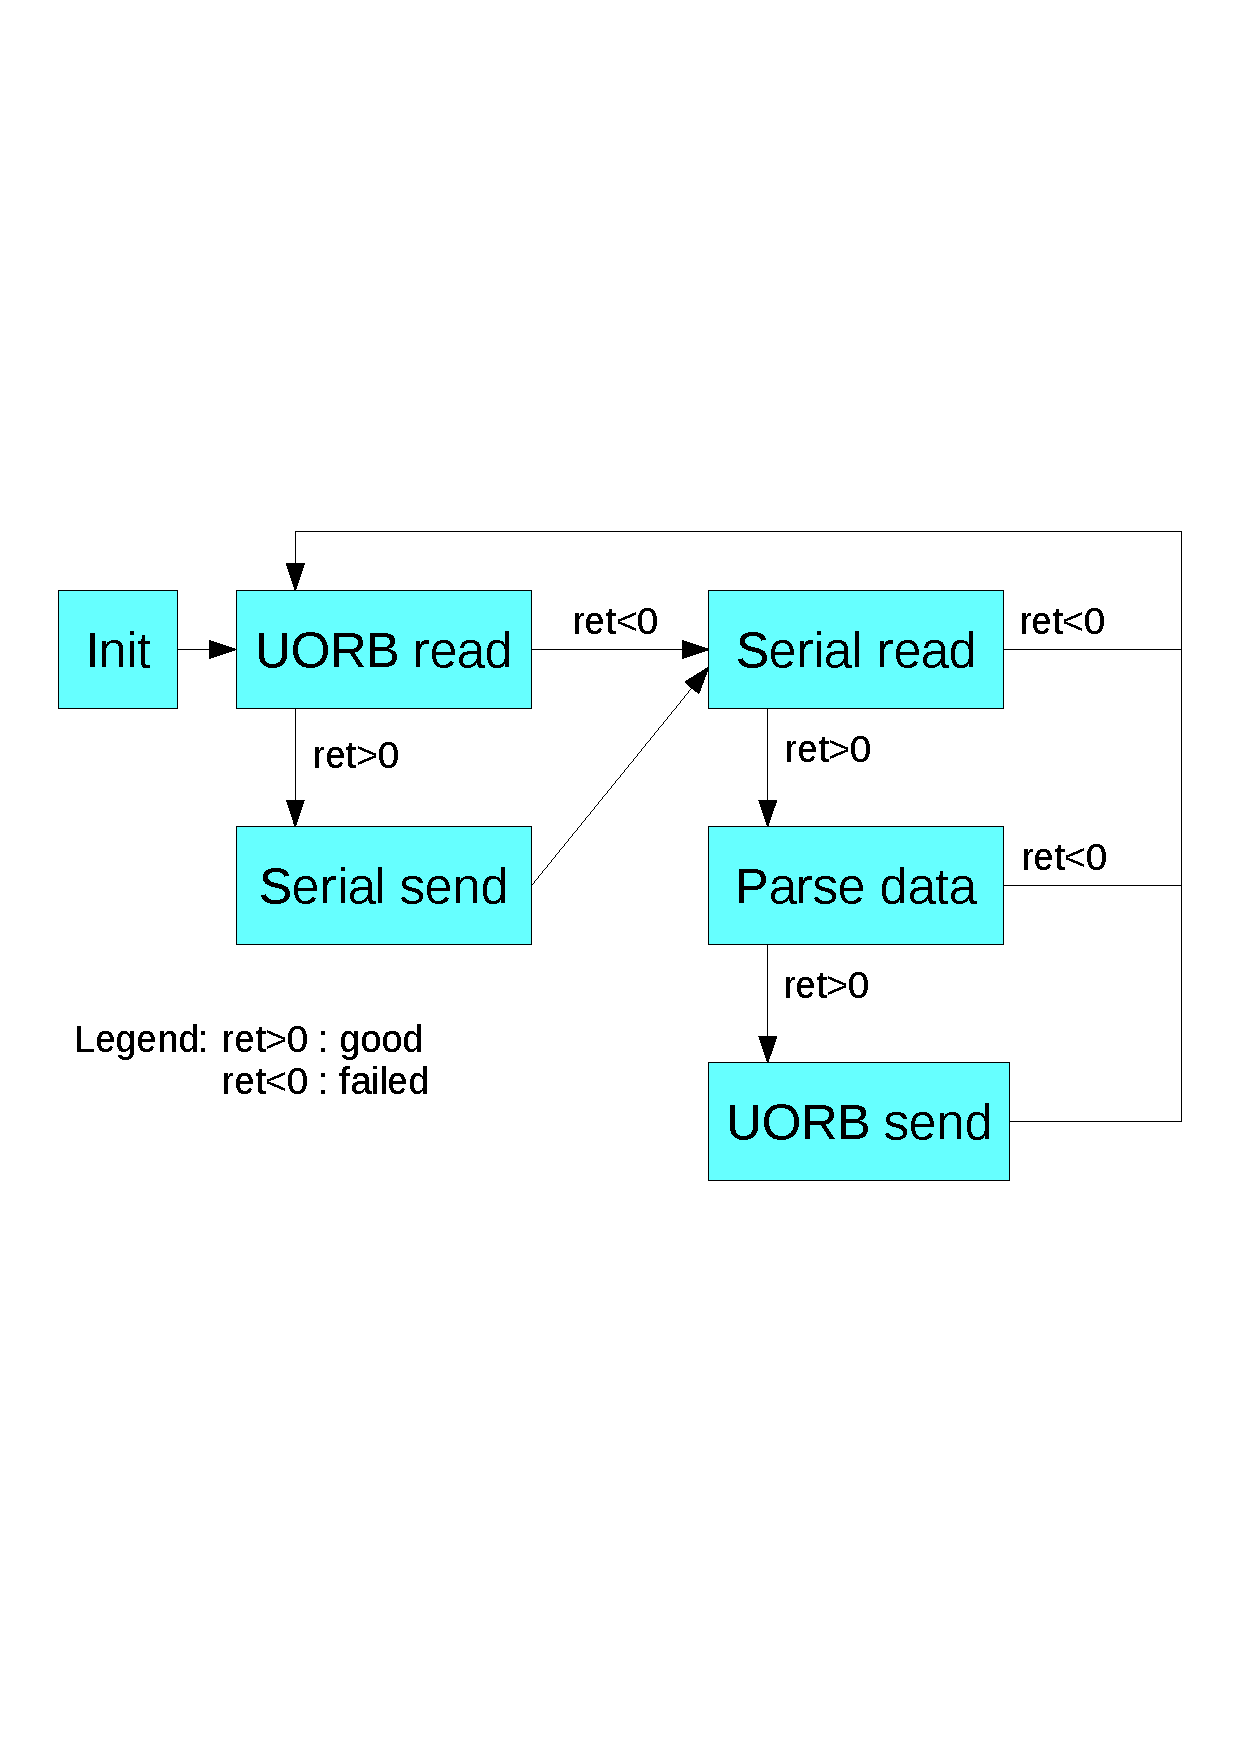
\includegraphics[scale=0.5, trim={1cm 9.5cm 1cm 9cm},clip]{pic/50_app/statemachine_thread.pdf}
  \caption{Statemachine Businesslogik}
  \label{fig:Statemachine Businesslogik}
  \end{center}
\end{figure}

\subsubsection{Parser}

\noindent Die Daten werden jeweils als Packet übertragen. Diese Struktur ist in Abbildung \ref{fig:packet} aufgezeigt. Eine Erweiterung wäre die ID der Payload zu übermitteln. Dadurch wüsste man, um welches uORB Topic es sich handelt.

\begin{figure}[ht]
  \begin{center}
  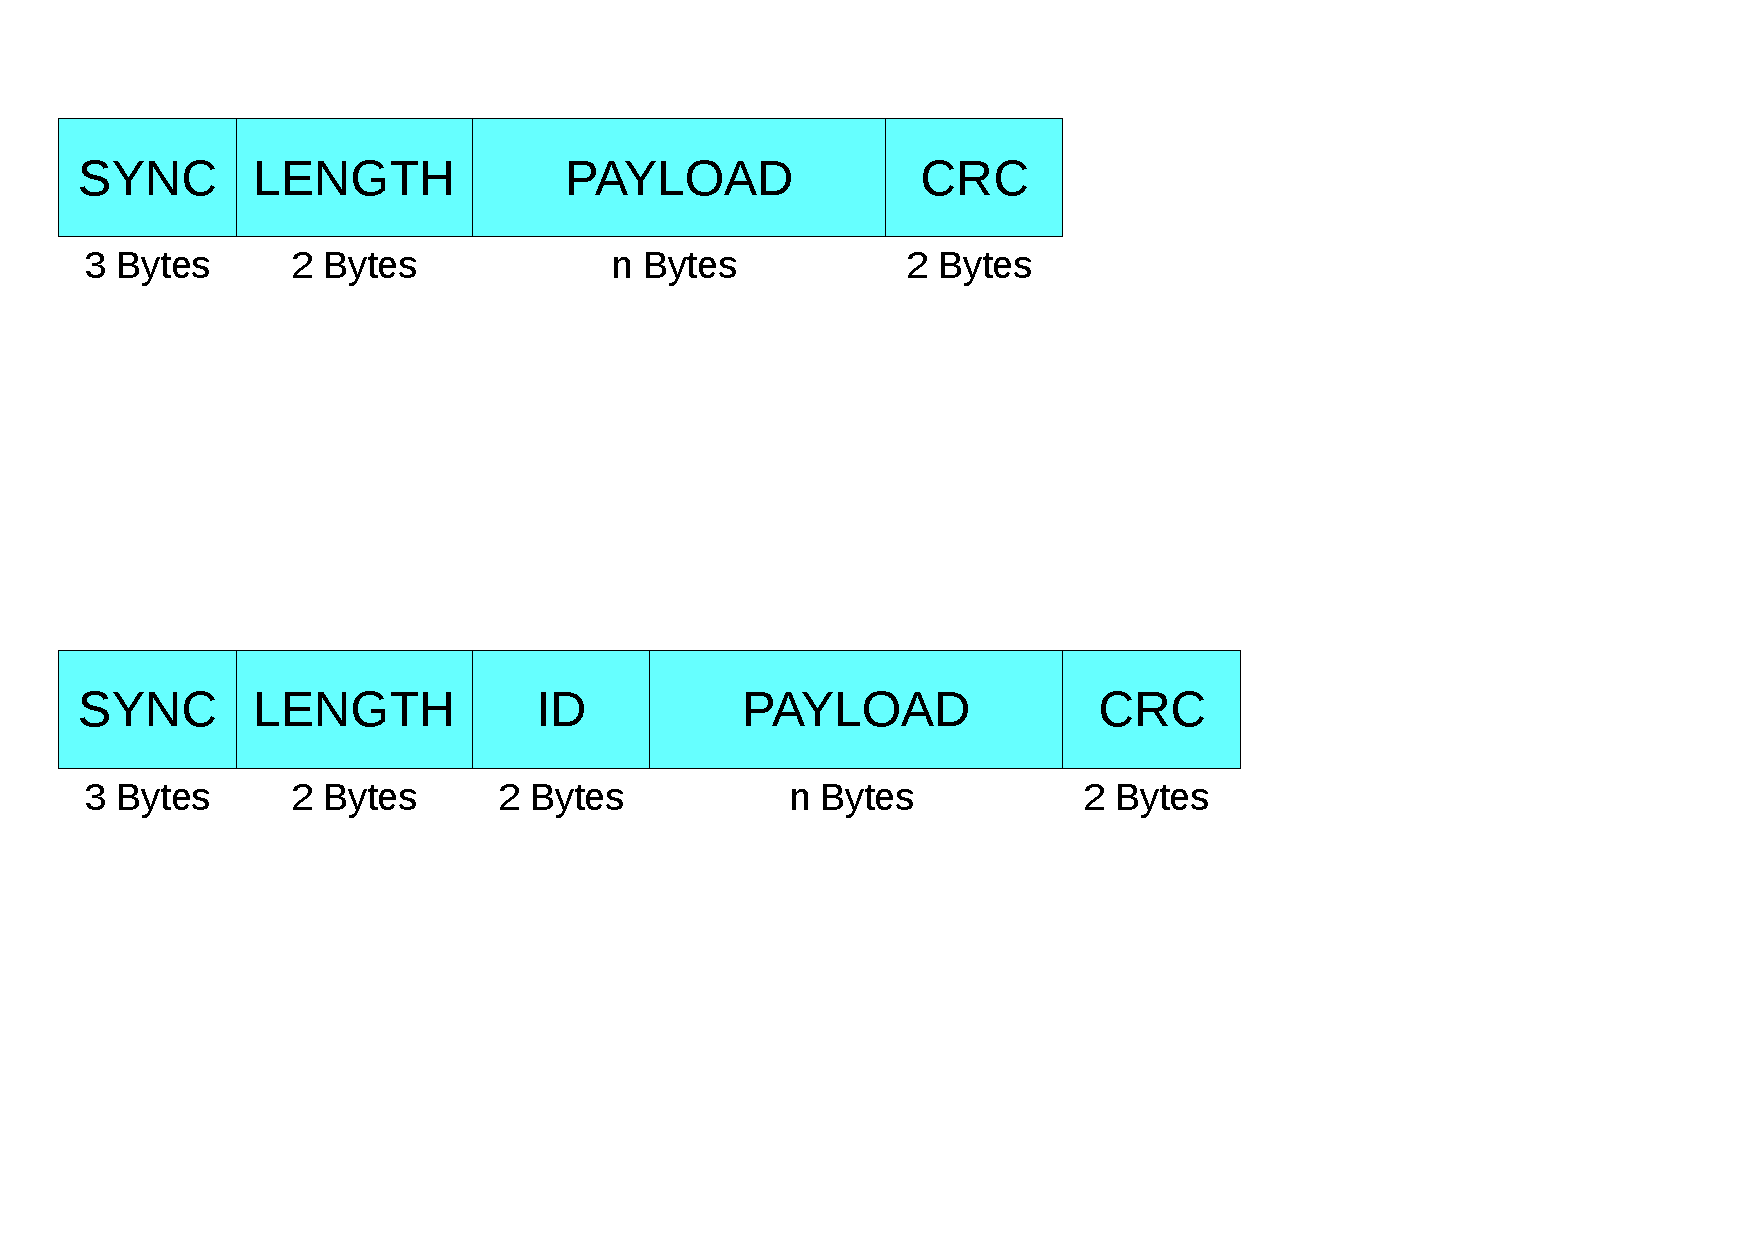
\includegraphics[scale=0.5, trim={1cm 16cm 11cm 1cm},clip]{pic/50_app/packet.pdf}
  \caption{Packet Struktur}
  \label{fig:packet}
  \end{center}
\end{figure}

\noindent Die bei den empfangenen Daten muss zuerst der Beginn festgelegt werden. Für dies wird eine Parser (Abbildung \ref{fig:Statemachine Parser} verwendet.


\begin{figure}[ht]
  \begin{center}
  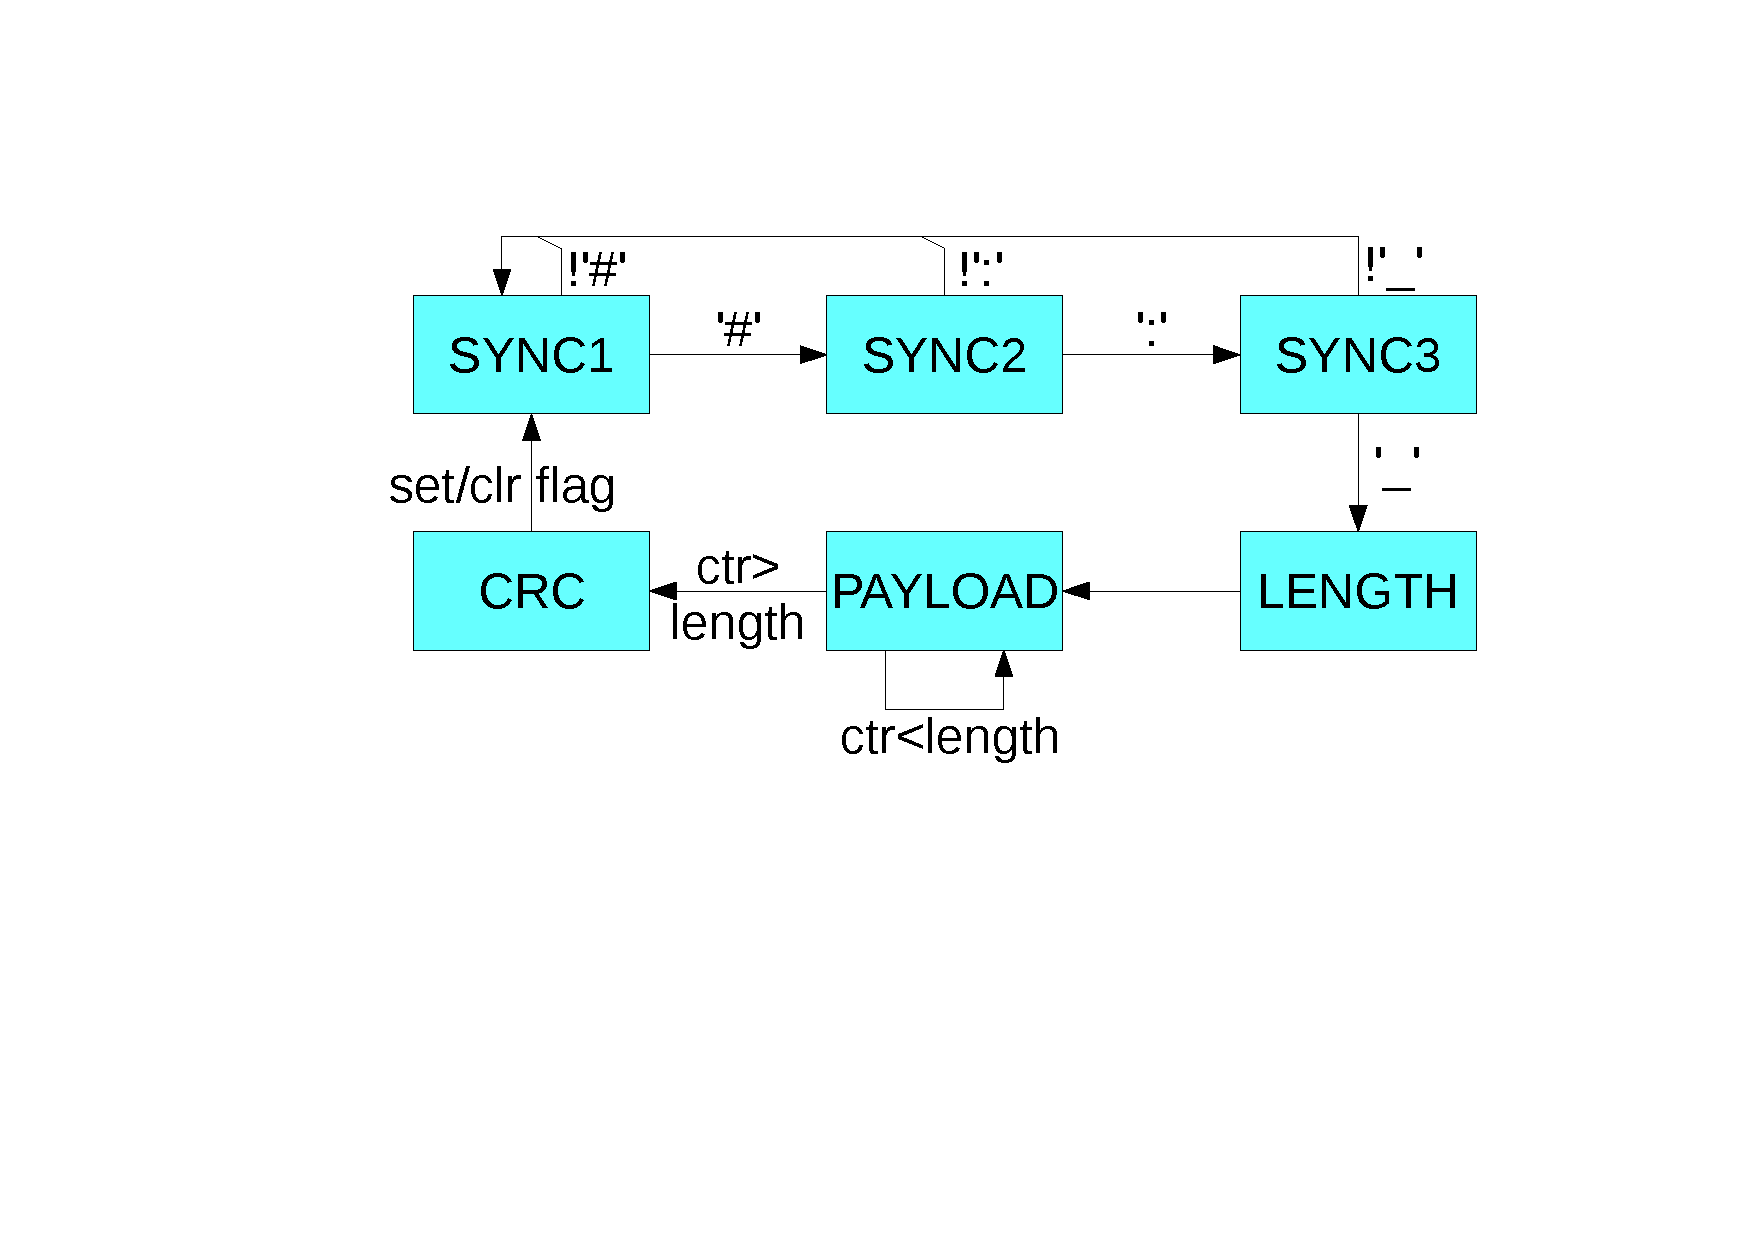
\includegraphics[scale=0.5, trim={1cm 20cm 1cm 1cm},clip]{pic/50_app/statemachine_parser.pdf}
  \caption{Statemachine Parser}
  \label{fig:Statemachine Parser}
  \end{center}
\end{figure}


\clearpage
